%%%%%%%%%%%%%%%%%%%%%%%%%%%%%%%%%%%%%%%%%%%%%%%%%%%%%%%%%%%%%%%%%%%%%%%%%%%%%%%%%%
\begin{frame}[fragile]\frametitle{}
\begin{center}
{\Large Graph Algorithms}
\end{center}
\end{frame}

%%%%%%%%%%%%%%%%%%%%%%%%%%%%%%%%%%%%%%%%%%%%%%%%%%%%%%%%%%%%%%%%%%%%%%%%%%%%%%%%%%
\begin{frame}[fragile]\frametitle{}
\begin{center}
{\Large Centrality }
\end{center}
\end{frame}


%%%%%%%%%%%%%%%%%%%%%%%%%%%%%%%%%%%%%%%%%%%%%%%%%%%%%%%%%%%%%%%%%%%%%%%%%%%%%%%%%%
\begin{frame}[fragile]\frametitle{What is Centrality?}
\begin{itemize}
\item In a knowledge graph, centrality measures the relative significance of individual nodes.
\item Centrality algorithms help identify key nodes that act as pivotal points of influence in the network.
\item It aids in understanding which nodes are critical for information flow and decision-making processes.
\item Some types of centrality: Degree centrality, Closeness centrality, and Betweenness centrality.
\item More algorithmic types are: Pagerank, Eigenvector
\end{itemize}
\end{frame}

%%%%%%%%%%%%%%%%%%%%%%%%%%%%%%%%%%%%%%%%%%%%%%%%%%%%%%%%%%%%%%%%%%%%%%%%%%%%%%%%%%
\begin{frame}[fragile]\frametitle{Graph Centralities}

  \begin{itemize}
    \item \textbf{Degree Centrality}
      \begin{itemize}
        \item Measures the number of direct connections a node has.
        \item A node with a higher degree centrality is more connected to other nodes.
      \end{itemize}
      % Degree Centrality: \\
      % $\text{Degree}(A) = 2, \text{Degree}(B) = 1, \text{Degree}(C) = 3, \text{Degree}(D) = 1$


    \item \textbf{Closeness Centrality}
      \begin{itemize}
        \item Measures how quickly a node can reach other nodes in the graph.
        \item A node with higher closeness centrality is closer to all other nodes.
      \end{itemize}
      % Closeness Centrality: \\
      % $\text{Closeness}(A) = \frac{1}{\frac{1}{2} + 1 + \frac{1}{2}} = \frac{4}{5}, \text{Closeness}(B) = \frac{4}{5}, \text{Closeness}(C) = \frac{4}{5}, \text{Closeness}(D) = \frac{4}{5}$

    \item \textbf{Betweenness Centrality}
      \begin{itemize}
        \item Measures how often a node appears on the shortest path between other nodes.
        \item A node with higher betweenness centrality acts as a bridge between different parts of the graph.
      \end{itemize}
      % Betweenness Centrality: \\
      % $\text{Betweenness}(A) = 0, \text{Betweenness}(B) = \frac{1}{2}, \text{Betweenness}(C) = \frac{1}{2}, \text{Betweenness}(D) = 0$
  \end{itemize}
   
\end{frame}

%%%%%%%%%%%%%%%%%%%%%%%%%%%%%%%%%%%%%%%%%%%%%%%%%%%%%%%%%%%%%%%%%%%%%%%%%%%%%%%%%%
\begin{frame}[fragile]\frametitle{The Power of PageRank}
\begin{itemize}
\item PageRank, developed by Google's Larry Page and Sergey Brin, revolutionized web search rankings.
\item Originally designed for web pages, PageRank extends to any interconnected network, including insurance-related data.
\item PageRank assigns importance scores to nodes based on incoming links from other important nodes.
\item Nodes with high PageRank are considered influential and contribute significantly to information dissemination.
\item In insurance, PageRank can identify influential policies, clients, or agents within the network.
\end{itemize}
\end{frame}

%%%%%%%%%%%%%%%%%%%%%%%%%%%%%%%%%%%%%%%%%%%%%%%%%%%%%%%%%%%%%%%%%%%%%%%%%%%%%%%%%%
\begin{frame}[fragile]\frametitle{PageRank Calculation}
\begin{enumerate}
\item Start with assigning an initial score to all nodes.
\item Iteratively update each node's score based on incoming links and their corresponding scores.
\item Continue the iterations until convergence (scores stabilize).
\item The final scores represent the PageRank values of the nodes.
\end{enumerate}

$score(v) = \frac{{(1 - \text{damping\_factor})}}{N} + \text{damping\_factor} \times \sum_{u \in G} \frac{\text{score}(u)}{\text{out\_degree}(u)}$

In this formula, \lstinline|damping_factor| represents the probability that a user continues to another page rather than following a link, and \lstinline|out_degree(u)| is the number of outgoing links from node u.
% \textbf{Note:} PageRank calculation involves matrix manipulation and eigenvector computations.
\end{frame}

%%%%%%%%%%%%%%%%%%%%%%%%%%%%%%%%%%%%%%%%%%%%%%%%%%%%%%%%%%%%%%%%%%%%%%%%%%%%%%%%%%
\begin{frame}[fragile]\frametitle{PageRank Pseudo-code}

\begin{lstlisting}[basicstyle=\tiny]
1. Initialize the score for each node in the graph:
   For each node v in G:
       score(v) = 1 / N
	   
2. Set damping factor (usually 0.85):
   damping_factor = 0.85
   
3. Set maximum number of iterations and tolerance:
   max_iterations = 1000
   tolerance = 0.0001
   
4. Repeat the following steps until convergence or max_iterations:
   For iteration = 1 to max_iterations:
   5. Create a copy of the current scores:
      For each node v in G:
          old_score(v) = score(v)
   6. Update the score for each node:
      For each node v in G:
          score(v) = (1 - damping_factor) / N + damping_factor * sum(score(u) / out_degree(u)) for all nodes u pointing to v
   7. Check for convergence:
      For each node v in G:
          If abs(score(v) - old_score(v)) < tolerance:
              Converged for node v
   8. If scores have converged for all nodes, break out of the loop
   
9. Normalize the final scores:
   total_score = sum(score(v)) for all nodes v
   For each node v in G:
       score(v) = score(v) / total_score
	   
10. Return the PageRank scores for each node.
\end{lstlisting}

\end{frame}

%%%%%%%%%%%%%%%%%%%%%%%%%%%%%%%%%%%%%%%%%%%%%%%%%%%%%%%%%%%
\begin{frame}[fragile]\frametitle{PageRank}

\begin{center}
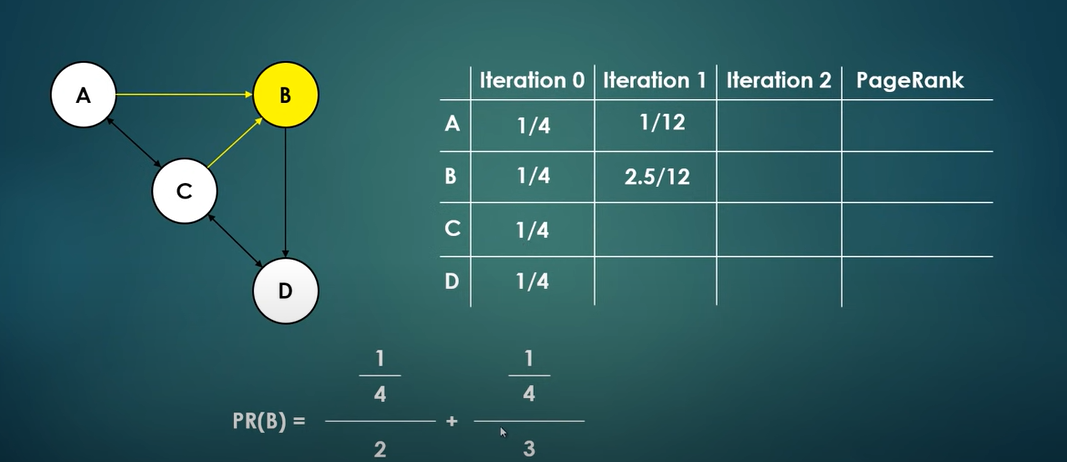
\includegraphics[width=0.6\linewidth,keepaspectratio]{pagerank}

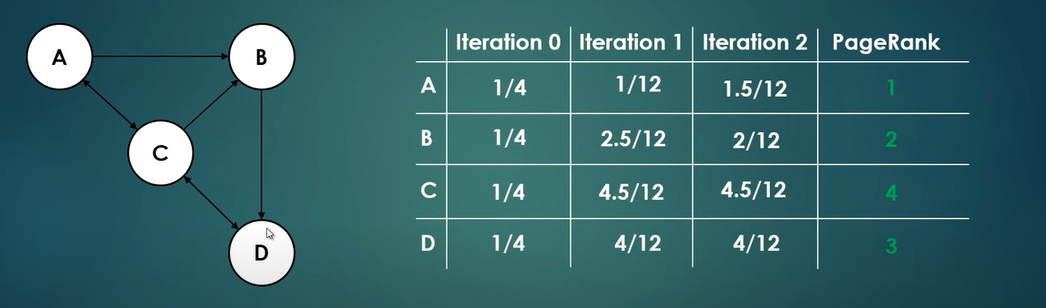
\includegraphics[width=0.6\linewidth,keepaspectratio]{pagerank1}

{\tiny (Ref: PageRank Algorithm - Example Global Software Support)}
\end{center}	  

Find nodes pointing to current node, to summation of those nodes previous page rank, divided by outgoing edges from that node
Start with initialization for each node, 1/n, n is total nodes. For A, lets consider C for now which is pointing to A. For C, ratio is 1/4 divided by 3 (C's outgoing links), so final is 1/12


\end{frame}


%%%%%%%%%%%%%%%%%%%%%%%%%%%%%%%%%%%%%%%%%%%%%%%%%%%%%%%%%%%%%%%%%%%%%%%%%%%%%%%%%%
\begin{frame}[fragile]\frametitle{PageRank code}

\begin{lstlisting}[basicstyle=\tiny]
def pagerank_centrality(graph, damping_factor=0.85, max_iterations=100, tolerance=1e-6):
    # Initialize PageRank scores for all nodes
    num_nodes = len(graph)
    pagerank = {node: 1 / num_nodes for node in graph}

    # Perform iterative PageRank calculation
    for _ in range(max_iterations):
        new_pagerank = {}
        for node in graph:
            incoming_nodes = [incoming_node for incoming_node in graph if node in graph[incoming_node]]
            incoming_pagerank = sum(pagerank[incoming_node] / len(graph[incoming_node]) for incoming_node in incoming_nodes)
            new_pagerank[node] = (1 - damping_factor) / num_nodes + damping_factor * incoming_pagerank
        # Check for convergence
        if all(abs(new_pagerank[node] - pagerank[node]) < tolerance for node in graph):
            break
        pagerank = new_pagerank
		
    return pagerank

\end{lstlisting}


\end{frame}


%%%%%%%%%%%%%%%%%%%%%%%%%%%%%%%%%%%%%%%%%%%%%%%%%%%%%%%%%%%%%%%%%%%%%%%%%%%%%%%%%%
\begin{frame}[fragile]\frametitle{PageRank code}

\begin{lstlisting}[basicstyle=\tiny]
# Example usage:
# Create a sample graph representing insurance data
graph = {
    1: [2, 3],
    2: [3],
    3: [4],
    4: [3]
}

# Compute the PageRank centrality scores
page_rank_centrality = pagerank_centrality(graph)

# Display the PageRank centrality scores for each node
print("PageRank Centrality Scores:")
for node, score in page_rank_centrality.items():
    print(f"Node {node}: {score:.4f}")

\end{lstlisting}


\end{frame}


%%%%%%%%%%%%%%%%%%%%%%%%%%%%%%%%%%%%%%%%%%%%%%%%%%%%%%%%%%%%%%%%%%%%%%%%%%%%%%%%%
\begin{frame}[fragile]\frametitle{Eigenvector Centrality}
\begin{itemize}
\item Degree centrality means the with who has more neighbors is more influential. But thats not the case in real life. So, a better measure is Eigenvector centrality as it incorporate influence of neighbors also.
\item Eigenvector centrality is another vital centrality measure used in various fields, including finance and insurance.
\item The centrality score of a node depends on the centrality of its neighboring nodes.
\item Nodes connected to other highly central nodes will have higher eigenvector centrality scores.
\item Eigenvector centrality can reveal nodes that have indirect influence through their connections.
\item In insurance, this can help identify key agents with a vast network of influential clients.
\end{itemize}
\end{frame}

%%%%%%%%%%%%%%%%%%%%%%%%%%%%%%%%%%%%%%%%%%%%%%%%%%%%%%%%%%%%%%%%%%%%%%%%%%%%%%%%%%
\begin{frame}[fragile]\frametitle{Eigenvector Centrality Calculation}
\begin{enumerate}
\item Start with initializing centrality scores for all nodes.
\item Update node scores iteratively based on their neighbors' scores.
\item NORMALIZE so that max becomes 1.
\item Continue the iterations until convergence.
\item The final scores represent the Eigenvector centrality values of the nodes.
\end{enumerate}

$score(v) = \sum_{u \in G} \frac{\text{score}(u)}{\text{degree}(u)}$


% \textbf{Note:} Eigenvector centrality relies on eigenvectors and requires special handling for large networks.
\end{frame}

%%%%%%%%%%%%%%%%%%%%%%%%%%%%%%%%%%%%%%%%%%%%%%%%%%%%%%%%%%%%%%%%%%%%%%%%%%%%%%%%%%
\begin{frame}[fragile]\frametitle{PageRank Pseudo-code}

\begin{lstlisting}[basicstyle=\tiny]
1. Initialize the score for each node in the graph:
   For each node v in G:
       score(v) = 1
	   
2. Set maximum number of iterations and tolerance:
   max_iterations = 1000
   tolerance = 0.0001
   
3. Repeat the following steps until convergence or max_iterations:
   For iteration = 1 to max_iterations:
   
   4. Create a copy of the current scores:
      For each node v in G:
          old_score(v) = score(v)
   5. Update the score for each node:
      For each node v in G:
          score(v) = sum(score(u) / degree(u)) for all nodes u adjacent to v
   6. Calculate the normalization factor (used to prevent score explosion):
      normalization_factor = max(score)
   7. Normalize the scores:
      For each node v in G:
          score(v) = score(v) / normalization_factor
   8. Check for convergence:
      For each node v in G:
          If abs(score(v) - old_score(v)) < tolerance:
              Converged for node v
   9. If scores have converged for all nodes, break out of the loop
   
10. Return the Eigenvector Centrality scores for each node.
\end{lstlisting}

\end{frame}

%%%%%%%%%%%%%%%%%%%%%%%%%%%%%%%%%%%%%%%%%%%%%%%%%%%%%%%%%%%
\begin{frame}[fragile]\frametitle{Eigenvector Centrality}

\begin{center}
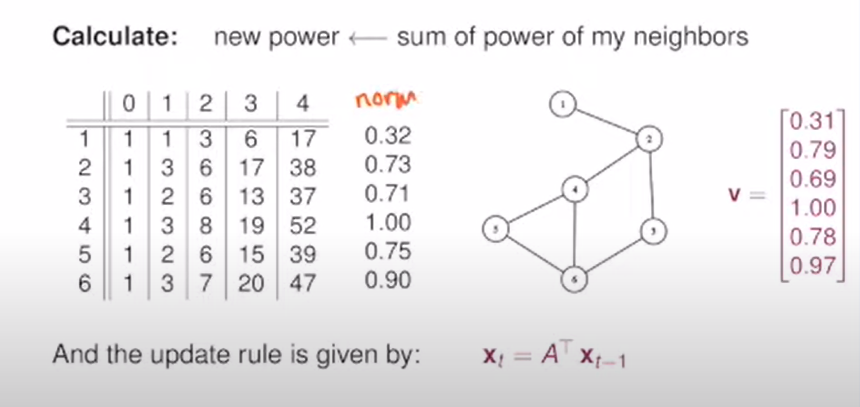
\includegraphics[width=0.8\linewidth,keepaspectratio]{eigcen}

{\tiny (Ref: NetSci 04-2 Eigenvector Centrality - Andrew Beveridge)}
\end{center}	  
\end{frame}

%%%%%%%%%%%%%%%%%%%%%%%%%%%%%%%%%%%%%%%%%%%%%%%%%%%%%%%%%%%%%%%%%%%%%%%%%%%%%%%%%%
\begin{frame}[fragile]\frametitle{Eigenvector Centrality Code}
\begin{lstlisting}[basicstyle=\tiny]
import numpy as np

def eigenvector_centrality(graph, max_iterations=100, tolerance=1e-6):
    # Initialize Eigenvector Centrality scores for all nodes
    num_nodes = len(graph)
    eigenvector_centrality = {node: 1 for node in graph}
    # Perform iterative Eigenvector Centrality calculation
    for _ in range(max_iterations):
        new_eigenvector_centrality = {}
        for node in graph:
            incoming_nodes = [incoming_node for incoming_node in graph if node in graph[incoming_node]]
            incoming_centrality_sum = sum(eigenvector_centrality[incoming_node] for incoming_node in incoming_nodes)
            new_eigenvector_centrality[node] = incoming_centrality_sum
        # Normalize the centrality scores
        norm = np.linalg.norm(list(new_eigenvector_centrality.values()))
        new_eigenvector_centrality = {node: score / norm for node, score in new_eigenvector_centrality.items()}
        # Check for convergence
        if all(abs(new_eigenvector_centrality[node] - eigenvector_centrality[node]) < tolerance for node in graph):
            break
        eigenvector_centrality = new_eigenvector_centrality
    return eigenvector_centrality
\end{lstlisting}

\end{frame}



%%%%%%%%%%%%%%%%%%%%%%%%%%%%%%%%%%%%%%%%%%%%%%%%%%%%%%%%%%%%%%%%%%%%%%%%%%%%%%%%%%
\begin{frame}[fragile]\frametitle{Eigenvector Centrality Code}
\begin{lstlisting}[basicstyle=\tiny]
# Example usage:
# Create a sample graph representing insurance data
graph = {
    1: [2, 3],
    2: [3],
    3: [4],
    4: [3]
}

# Compute the Eigenvector Centrality scores
eigenvector_centrality_scores = eigenvector_centrality(graph)

# Display the Eigenvector Centrality scores for each node
print("Eigenvector Centrality Scores:")
for node, score in eigenvector_centrality_scores.items():
    print(f"Node {node}: {score:.4f}")

\end{lstlisting}

\end{frame}


%%%%%%%%%%%%%%%%%%%%%%%%%%%%%%%%%%%%%%%%%%%%%%%%%%%%%%%%%%%%%%%%%%%%%%%%%%%%%%%%%%
\begin{frame}[fragile]\frametitle{Real-world Insurance Applications}
\begin{itemize}
\item Centrality algorithms find numerous applications in the insurance industry:
\begin{itemize}
\item Identifying key policyholders for targeted marketing campaigns.
\item Assessing agents' influence and performance within the network.
\item Detecting potential fraud by analyzing suspicious connections.
\item Enhancing risk assessment by understanding complex interdependencies.
\item Improving customer service through personalized recommendations.
\end{itemize}
\item Centrality provides actionable insights for better decision-making and operational efficiency.
\end{itemize}
\end{frame}

%%%%%%%%%%%%%%%%%%%%%%%%%%%%%%%%%%%%%%%%%%%%%%%%%%%%%%%%%%%%%%%%%%%%%%%%%%%%%%%%%%
\begin{frame}[fragile]\frametitle{Data Challenges and Ethical Considerations}
\begin{itemize}
\item Insurance companies handle vast amounts of sensitive data, requiring secure handling.
\item Ensuring data privacy and compliance with regulations is critical when applying centrality algorithms.
\item High-quality data and accurate network representations are essential for meaningful results.
\item Ethical considerations include avoiding bias and discrimination in centrality-based decisions.
\item Striking the right balance between data-driven insights and responsible use of centrality is paramount.
\end{itemize}
\end{frame}

%%%%%%%%%%%%%%%%%%%%%%%%%%%%%%%%%%%%%%%%%%%%%%%%%%%%%%%%%%%%%%%%%%%%%%%%%%%%%%%%%%
\begin{frame}[fragile]\frametitle{Embracing the Power of Centrality}
\begin{itemize}
\item Leveraging centrality algorithms can provide a competitive advantage in the insurance industry.
\item Identifying key influencers and critical nodes helps optimize operations and mitigate risks.
\item Centrality complements traditional analytics, leading to better data-driven strategies.
\item Continuous refinement of centrality models enhances decision-making capabilities.
\item Stay ahead of the curve by embracing graph centrality in your insurance workflows.
\end{itemize}
\end{frame}

%%%%%%%%%%%%%%%%%%%%%%%%%%%%%%%%%%%%%%%%%%%%%%%%%%%%%%%%%%%%%%%%%%%%%%%%%%%%%%%%%%
\begin{frame}[fragile]\frametitle{}
\begin{center}
{\Large Similarity}
\end{center}
\end{frame}

%%%%%%%%%%%%%%%%%%%%%%%%%%%%%%%%%%%%%%%%%%%%%%%%%%%%%%%%%%%%%%%%%%%%%%%%%%%%%%%%%%
\begin{frame}[fragile]\frametitle{Understanding Similarity}
\begin{itemize}
\item In the insurance domain, data is often represented as a knowledge graph.
\item Graph Similarity measures quantify the likeness between nodes or subgraphs within this graph.
\item Similarity algorithms enable us to find nodes or entities that share common characteristics or behaviors.
\item It plays a crucial role in recommendation systems, fraud detection, and customer segmentation.
\item Let's explore one powerful subtype of Graph Similarity: K-Nearest Neighbors (K-NN).
\end{itemize}
\end{frame}

%%%%%%%%%%%%%%%%%%%%%%%%%%%%%%%%%%%%%%%%%%%%%%%%%%%%%%%%%%%%%%%%%%%%%%%%%%%%%%%%%%
\begin{frame}[fragile]\frametitle{Introducing K-Nearest Neighbors (K-NN)}
\begin{itemize}
\item K-NN is a popular algorithm used in various machine learning tasks, including similarity analysis.
\item It is a non-parametric and lazy learning method, making it suitable for dynamic and changing insurance data.
\item K-NN finds K nearest neighbors to a given node based on a similarity metric, such as Euclidean distance or Jaccard index.
\item The algorithm can be adapted to various use cases, such as finding similar clients for personalized recommendations.
\item Next, we'll dive into the mechanics of K-NN and see how it works in the insurance context.
\end{itemize}
\end{frame}

%%%%%%%%%%%%%%%%%%%%%%%%%%%%%%%%%%%%%%%%%%%%%%%%%%%%%%%%%%%%%%%%%%%%%%%%%%%%%%%%%%
\begin{frame}[fragile]\frametitle{How K-NN Works}
\begin{enumerate}
\item Start with defining a similarity metric to measure the distance between nodes or entities.
\item Select the value of K (number of neighbors) based on the problem's requirements and data size.
\item For each node in the graph, find its K nearest neighbors based on the similarity metric.
\item Based on the K neighbors, the node's attributes or behavior can be predicted or analyzed.
\item K-NN is intuitive, easy to implement, and doesn't require a training phase.
\end{enumerate}
\end{frame}

%%%%%%%%%%%%%%%%%%%%%%%%%%%%%%%%%%%%%%%%%%%%%%%%%%%%%%%%%%%%%%%%%%%%%%%%%%%%%%%%%%
\begin{frame}[fragile]\frametitle{KNN Pseudo-code}

\begin{lstlisting}[basicstyle=\tiny]
Input: Graph G with N nodes, target node v, and parameter K
Output: List of K-nearest neighbors of the target node v

KNN Algorithm for Graphs:
1. Compute the similarity score between the target node v and all other nodes in the graph:
   For each node u in G:
       similarity(u, v) = [Some similarity metric between u and v]

2. Sort the nodes based on their similarity scores in descending order:
   SortedNodes = Sort(G.nodes, key=lambda u: similarity(u, v), reverse=True)

3. Select the top K nodes with the highest similarity scores as the K-nearest neighbors:
   KNearestNeighbors = SortedNodes[:K]

4. Return the list of K-nearest neighbors KNearestNeighbors.
\end{lstlisting}

\end{frame}

%%%%%%%%%%%%%%%%%%%%%%%%%%%%%%%%%%%%%%%%%%%%%%%%%%%%%%%%%%%%%%%%%%%%%%%%%%%%%%%%%%
\begin{frame}[fragile]\frametitle{K-NN code}
\begin{lstlisting}[basicstyle=\tiny]
import numpy as np
from collections import defaultdict

def euclidean_distance(a, b):
    return np.sqrt(np.sum((a - b) ** 2))

def k_nearest_neighbors(data, labels, new_data_point, k=3):
    distances = defaultdict(list)

    for i, data_point in enumerate(data):
        distance = euclidean_distance(data_point, new_data_point)
        distances[distance].append(i)

    k_nearest_indices = sorted(distances.keys())[:k]
    k_nearest_labels = [labels[i] for index in k_nearest_indices for i in distances[index]]

    return max(set(k_nearest_labels), key=k_nearest_labels.count)
\end{lstlisting}

\end{frame}



%%%%%%%%%%%%%%%%%%%%%%%%%%%%%%%%%%%%%%%%%%%%%%%%%%%%%%%%%%%%%%%%%%%%%%%%%%%%%%%%%%
\begin{frame}[fragile]\frametitle{K-NN code}

\begin{lstlisting}[basicstyle=\tiny]
# Example usage:
# Sample insurance data with attributes (age, income)
data = np.array([[25, 50000], [30, 60000], [40, 70000], [45, 80000]])
labels = np.array(['low risk', 'medium risk', 'high risk', 'low risk'])

# New data point to classify
new_data_point = np.array([35, 75000])

# Classify the new data point using K-Nearest Neighbors
predicted_label = k_nearest_neighbors(data, labels, new_data_point)

print(f"Predicted label for new data point: {predicted_label}")

\end{lstlisting}

\end{frame}

%%%%%%%%%%%%%%%%%%%%%%%%%%%%%%%%%%%%%%%%%%%%%%%%%%%%%%%%%%%%%%%%%%%%%%%%%%%%%%%%%%
\begin{frame}[fragile]\frametitle{Real-world Applications in Insurance}
\begin{itemize}
\item K-NN has several practical applications in the insurance industry:
\begin{itemize}
\item Customer Segmentation: Grouping policyholders with similar needs for targeted marketing.
\item Fraud Detection: Identifying anomalous behavior based on the behavior of similar clients.
\item Risk Assessment: Predicting risk profiles based on similarities with historical claims data.
\item Customer Lifetime Value: Estimating the long-term value of clients based on similar customer behaviors.
\item Cross-selling: Recommending relevant insurance products to clients with similar preferences.
\end{itemize}
\item K-NN empowers insurers to offer personalized services and make data-driven decisions.
\end{itemize}
\end{frame}

%%%%%%%%%%%%%%%%%%%%%%%%%%%%%%%%%%%%%%%%%%%%%%%%%%%%%%%%%%%%%%%%%%%%%%%%%%%%%%%%%%
\begin{frame}[fragile]\frametitle{Challenges and Considerations}
\begin{itemize}
\item While K-NN offers valuable insights, there are certain challenges and considerations to keep in mind:
\begin{itemize}
\item Choice of Similarity Metric: Selecting an appropriate similarity measure is crucial for accurate results.
\item Curse of Dimensionality: High-dimensional data can impact the algorithm's performance.
\item Scalability: As the dataset grows, computation time may increase, affecting real-time applications.
\item Data Quality: Inaccurate or incomplete data can lead to misleading similarity results.
\item Bias: Bias in the data can affect the fairness of recommendations and decisions.
\end{itemize}
\item Addressing these challenges ensures the responsible and effective use of K-NN in insurance applications.
\end{itemize}
\end{frame}

%%%%%%%%%%%%%%%%%%%%%%%%%%%%%%%%%%%%%%%%%%%%%%%%%%%%%%%%%%%%%%%%%%%%%%%%%%%%%%%%%%
\begin{frame}[fragile]\frametitle{Integrating Graph Similarity in Workflows}
\begin{itemize}
\item Incorporating Graph Similarity and K-NN into your insurance workflows can yield significant benefits:
\begin{itemize}
\item Enhanced Customer Experience: Personalized services and tailored product recommendations.
\item Improved Risk Management: Early fraud detection and accurate risk assessment.
\item Optimal Resource Allocation: Targeted marketing efforts and efficient cross-selling.
\item Better Decision-making: Data-driven insights for strategic planning and policy optimization.
\end{itemize}
\item By leveraging these algorithms, insurers can stay competitive and agile in a dynamic market landscape.
\end{itemize}
\end{frame}

%%%%%%%%%%%%%%%%%%%%%%%%%%%%%%%%%%%%%%%%%%%%%%%%%%%%%%%%%%%%%%%%%%%%%%%%%%%%%%%%%%
\begin{frame}[fragile]\frametitle{}
\begin{center}
{\Large Pathfinding}
\end{center}
\end{frame}

%%%%%%%%%%%%%%%%%%%%%%%%%%%%%%%%%%%%%%%%%%%%%%%%%%%%%%%%%%%%%%%%%%%%%%%%%%%%%%%%%%
\begin{frame}[fragile]\frametitle{Understanding Graph Pathfinding}
\begin{itemize}
\item In the insurance industry, knowledge graphs model complex relationships between entities like policies, claims, and customers.
\item Pathfinding algorithms help us navigate this interconnected web and find the most efficient routes between nodes.
\item The fundamental problem is finding the shortest or most optimal path between two nodes in the graph.
\item These algorithms have significant implications for claim processing, cost optimization, and even customer satisfaction.
\item Now, let's delve deeper into the magic of Shortest Path algorithms.
\end{itemize}
\end{frame}

%%%%%%%%%%%%%%%%%%%%%%%%%%%%%%%%%%%%%%%%%%%%%%%%%%%%%%%%%%%%%%%%%%%%%%%%%%%%%%%%%%
\begin{frame}[fragile]\frametitle{Introducing Shortest Path Algorithms}
\begin{itemize}
\item Shortest Path algorithms are a class of graph algorithms that focus on finding the most efficient route between two nodes.
\item These algorithms are vital in scenarios like:
\begin{itemize}
\item Determining the shortest route for claims processing, reducing turnaround time.
\item Identifying the quickest path for field agents to reach clients in emergencies.
\item Minimizing operational costs by optimizing logistics and resource allocation.
\item Evaluating risk exposure by analyzing paths through interconnected policies.
\end{itemize}
\item Next, we'll explore two popular Shortest Path algorithms: Dijkstra's algorithm and A* algorithm.
\end{itemize}
\end{frame}

%%%%%%%%%%%%%%%%%%%%%%%%%%%%%%%%%%%%%%%%%%%%%%%%%%%%%%%%%%%%%%%%%%%%%%%%%%%%%%%%%%
\begin{frame}[fragile]\frametitle{Dijkstra's Algorithm}
\begin{itemize}
\item Dijkstra's algorithm, proposed by Edsger W. Dijkstra in 1956, is a widely used shortest path algorithm.
\item It guarantees finding the shortest path in non-negative weighted graphs.
\item Dijkstra's algorithm is employed in various insurance-related applications, such as optimizing claim processing workflows.
\item This algorithm is efficient for finding the shortest path from a single source to all other nodes in the graph.
\item Let's see how Dijkstra's algorithm works in action.
\end{itemize}
\end{frame}

%%%%%%%%%%%%%%%%%%%%%%%%%%%%%%%%%%%%%%%%%%%%%%%%%%%%%%%%%%%%%%%%%%%%%%%%%%%%%%%%%%
\begin{frame}[fragile]\frametitle{How Dijkstra's Algorithm Works}
\begin{enumerate}
\item Start by initializing distances from the source node to all other nodes as infinity.
\item Set the distance from the source node to itself as zero.
\item Repeatedly select the node with the smallest distance from the source (not yet visited).
\item Update the distances to its neighbors if a shorter path is found.
\item Continue until all nodes are visited and their shortest distances are determined.
\end{enumerate}
\end{frame}

%%%%%%%%%%%%%%%%%%%%%%%%%%%%%%%%%%%%%%%%%%%%%%%%%%%%%%%%%%%%%%%%%%%%%%%%%%%%%%%%%%
\begin{frame}[fragile]\frametitle{Dijkstra's Algorithm Pseudo-code}

\begin{lstlisting}[basicstyle=\tiny]
Input: Graph G with N nodes, source node s
Output: Shortest path distances from the source node s to all other nodes

Dijkstra Algorithm:
1. Initialize the distance scores for all nodes in the graph:
   For each node v in G:
       distance(v) = infinity

2. Set the distance score of the source node s to zero:
   distance(s) = 0

3. Create an empty priority queue Q to store nodes and their distance scores.

4. Add the source node s to the priority queue with a distance of zero.

5. While the priority queue Q is not empty:
   a. Dequeue the node u with the minimum distance score from Q.
   b. For each neighbor v of node u:
      i. Calculate the tentative distance from the source node s to node v:
         tentative_distance = distance(u) + weight(u, v)  // weight(u, v) is the weight of the edge from u to v.
      ii. If tentative_distance is less than the current distance(v), update distance(v) to the tentative_distance.
      iii. Enqueue node v into Q with the updated distance(v).

6. Return the shortest path distances distance(v) for all nodes v in G.
\end{lstlisting}

\end{frame}

%%%%%%%%%%%%%%%%%%%%%%%%%%%%%%%%%%%%%%%%%%%%%%%%%%%%%%%%%%%%%%%%%%%%%%%%%%%%%%%%%%
\begin{frame}[fragile]\frametitle{Dijkstra's Algorithm code}

\begin{lstlisting}[basicstyle=\tiny]
import math

def dijkstra(graph, start_node):
    distances = {node: math.inf for node in graph}
    distances[start_node] = 0

    visited = set()
    while len(visited) < len(graph):
        # Find the node with the minimum distance
        min_node = None
        for node in graph:
            if node not in visited and (min_node is None or distances[node] < distances[min_node]):
                min_node = node

        # Calculate distances to neighbors from the current node
        for neighbor, weight in graph[min_node].items():
            total_distance = distances[min_node] + weight
            if total_distance < distances[neighbor]:
                distances[neighbor] = total_distance

        visited.add(min_node)

    return distances
\end{lstlisting}

\end{frame}


%%%%%%%%%%%%%%%%%%%%%%%%%%%%%%%%%%%%%%%%%%%%%%%%%%%%%%%%%%%%%%%%%%%%%%%%%%%%%%%%%%
\begin{frame}[fragile]\frametitle{Dijkstra's Algorithm code}

\begin{lstlisting}[basicstyle=\tiny]
# Example usage:
# Create a sample graph representing insurance data with weighted edges
graph = {
    'A': {'B': 5, 'C': 3},
    'B': {'C': 2, 'D': 4},
    'C': {'D': 6, 'E': 8},
    'D': {'E': 3},
    'E': {}
}

# Find the shortest path distances from node 'A'
shortest_distances = dijkstra(graph, 'A')

# Display the shortest path distances from node 'A' to other nodes
print("Shortest Path Distances from Node 'A':")
for node, distance in shortest_distances.items():
    print(f"To node '{node}': {distance}")

\end{lstlisting}
\end{frame}

%%%%%%%%%%%%%%%%%%%%%%%%%%%%%%%%%%%%%%%%%%%%%%%%%%%%%%%%%%%%%%%%%%%%%%%%%%%%%%%%%%
\begin{frame}[fragile]\frametitle{Usage}
\begin{enumerate}
\item In the insurance domain, this can be used for route optimization, claims processing, or finding the most efficient way to reach policyholders in case of emergencies.
\item  Claims Processing: Suppose an insurance company receives a claim from a policyholder located in a remote area. Using Dijkstra's algorithm, the insurer can find the shortest path to reach the insured's location, minimizing response time and ensuring prompt assistance.
\end{enumerate}
\end{frame}



%%%%%%%%%%%%%%%%%%%%%%%%%%%%%%%%%%%%%%%%%%%%%%%%%%%%%%%%%%%%%%%%%%%%%%%%%%%%%%%%%%
\begin{frame}[fragile]\frametitle{A* Algorithm}
\begin{itemize}
\item The A* algorithm is a popular extension of Dijkstra's algorithm and is widely used in pathfinding problems.
\item It employs a heuristic function to guide the search and improve efficiency.
\item A* is particularly useful in scenarios where we need to find the shortest path from a source to a destination node.
\item In insurance, the A* algorithm can optimize navigation for agents visiting clients in different locations.
\item Let's uncover the mechanics of the A* algorithm.
\end{itemize}
\end{frame}

%%%%%%%%%%%%%%%%%%%%%%%%%%%%%%%%%%%%%%%%%%%%%%%%%%%%%%%%%%%%%%%%%%%%%%%%%%%%%%%%%%
\begin{frame}[fragile]\frametitle{How A* Algorithm Works}
\begin{enumerate}
\item Similar to Dijkstra's algorithm, initialize distances from the source node to all others as infinity.
\item Set the distance from the source node to itself as zero.
\item In addition to the distance, compute a heuristic value (estimated distance) from each node to the destination node.
\item Repeatedly select the node with the smallest sum of distance and heuristic value (not yet visited).
\item Update the distances to its neighbors if a shorter path is found, considering the heuristic value.
\item Continue until the destination node is reached, and the shortest path is determined.
\end{enumerate}
\end{frame}

%%%%%%%%%%%%%%%%%%%%%%%%%%%%%%%%%%%%%%%%%%%%%%%%%%%%%%%%%%%%%%%%%%%%%%%%%%%%%%%%%%
\begin{frame}[fragile]\frametitle{A star Algorithm Pseudo-code}

\begin{lstlisting}[basicstyle=\tiny]
Input: Graph G with N nodes, source node s, target node t
Output: Shortest path from source node s to target node t

A* Algorithm:
1. Initialize the G-Score and F-Score for all nodes in the graph:
   For each node v in G:
       G-Score(v) = infinity  // The actual cost of the cheapest path from s to v
       F-Score(v) = infinity  // G-Score(v) + heuristic_estimate(v, t)

2. Set the G-Score of the source node s to zero:
   G-Score(s) = 0

3. Set the F-Score of the source node s using the heuristic estimate:
   F-Score(s) = heuristic_estimate(s, t)

4. Create an open set to store nodes to be evaluated. Initially, it contains only the source node s.

5. While the open set is not empty:
   a. Dequeue the node u with the lowest F-Score from the open set.
   b. If u is the target node t, reconstruct the path from s to t and return it.
   c. For each neighbor v of node u:
      i. Calculate the tentative G-Score for node v:
         tentative_G_Score = G-Score(u) + weight(u, v)  // weight(u, v) is the weight of the edge from u to v.
      ii. If tentative_G_Score is less than G-Score(v), update G-Score(v) to tentative_G_Score and set F-Score(v) using the heuristic estimate:
          G-Score(v) = tentative_G_Score
          F-Score(v) = G-Score(v) + heuristic_estimate(v, t)
      iii. If v is not already in the open set, enqueue it.

6. No path from s to t is found, return failure.
\end{lstlisting}

\end{frame}


%%%%%%%%%%%%%%%%%%%%%%%%%%%%%%%%%%%%%%%%%%%%%%%%%%%%%%%%%%%%%%%%%%%%%%%%%%%%%%%%%%
\begin{frame}[fragile]\frametitle{A* Algorithm code}

\begin{lstlisting}[basicstyle=\tiny]
import math

def euclidean_distance(a, b):
    return math.sqrt((a[0] - b[0])**2 + (a[1] - b[1])**2)

def reconstruct_path(graph, start, goal):
    current = goal
    path = [current]
    while current != start:
        current = min(graph[current], key=lambda node: g_score[node] + euclidean_distance(node, goal))
        path.append(current)
    return list(reversed(path))
	
def a_star(graph, start, goal):
    open_set = set([start])
    closed_set = set()
    
    g_score = {node: math.inf for node in graph}
    g_score[start] = 0
    
    f_score = {node: math.inf for node in graph}
    f_score[start] = euclidean_distance(start, goal)
	
\end{lstlisting}

\end{frame}


%%%%%%%%%%%%%%%%%%%%%%%%%%%%%%%%%%%%%%%%%%%%%%%%%%%%%%%%%%%%%%%%%%%%%%%%%%%%%%%%%%
\begin{frame}[fragile]\frametitle{A* Algorithm code}

\begin{lstlisting}[basicstyle=\tiny]

    
    while open_set:
        current = min(open_set, key=lambda node: f_score[node])
        if current == goal:
            return reconstruct_path(graph, start, goal)
        open_set.remove(current)
        closed_set.add(current)
        
        for neighbor, cost in graph[current].items():
            if neighbor in closed_set:
                continue
            tentative_g_score = g_score[current] + cost
            if neighbor not in open_set:
                open_set.add(neighbor)
            elif tentative_g_score >= g_score[neighbor]:
                continue
            g_score[neighbor] = tentative_g_score
            f_score[neighbor] = g_score[neighbor] + euclidean_distance(neighbor, goal)
    return None
\end{lstlisting}

\end{frame}


%%%%%%%%%%%%%%%%%%%%%%%%%%%%%%%%%%%%%%%%%%%%%%%%%%%%%%%%%%%%%%%%%%%%%%%%%%%%%%%%%%
\begin{frame}[fragile]\frametitle{A* Algorithm code}

\begin{lstlisting}[basicstyle=\tiny]
# Example usage:
# Create a sample graph representing insurance data with weighted edges (Euclidean distances)
graph = {
    (0, 0): {(1, 1): 1.41, (0, 1): 1.0},
    (1, 1): {(2, 2): 1.41, (1, 0): 1.0},
    (0, 1): {(0, 2): 1.0},
    (2, 2): {(2, 3): 1.0},
    (0, 2): {(1, 2): 1.0},
    (1, 2): {(2, 2): 1.0, (1, 3): 1.0},
    (2, 3): {}
}

# Define start and goal nodes
start_node = (0, 0)
goal_node = (2, 3)

# Find the shortest path using A* algorithm
shortest_path = a_star(graph, start_node, goal_node)

# Display the shortest path
print("Shortest Path from", start_node, "to", goal_node, ":", shortest_path)
\end{lstlisting}
\end{frame}


%%%%%%%%%%%%%%%%%%%%%%%%%%%%%%%%%%%%%%%%%%%%%%%%%%%%%%%%%%%%%%%%%%%%%%%%%%%%%%%%%%
\begin{frame}[fragile]\frametitle{Real-world Insurance Applications}
\begin{itemize}
\item Shortest Path algorithms offer numerous practical applications in the insurance industry:
\begin{itemize}
\item Optimizing claims processing by finding the most efficient route through interconnected policies and claims data.
\item Streamlining field agent operations for faster response times and improved customer service.
\item Analyzing risk exposure and dependencies between different policies and insurance products.
\item Minimizing operational costs by optimizing resource allocation and logistics.
\end{itemize}
\item These algorithms empower insurers to make data-driven decisions, enhancing efficiency and customer satisfaction.
\end{itemize}
\end{frame}

%%%%%%%%%%%%%%%%%%%%%%%%%%%%%%%%%%%%%%%%%%%%%%%%%%%%%%%%%%%%%%%%%%%%%%%%%%%%%%%%%%
\begin{frame}[fragile]\frametitle{Challenges and Considerations}
\begin{itemize}
\item While Shortest Path algorithms offer invaluable insights, there are challenges and considerations to address:
\begin{itemize}
\item Data Accuracy: Reliable data is essential to ensure the accuracy of the shortest path.
\item Dynamic Environments: Insurance data is ever-changing; algorithms should adapt accordingly.
\item Scalability: As the graph size grows, computational complexity can impact real-time applications.
\item Heuristic Selection: Choosing appropriate heuristics affects the algorithm's efficiency and accuracy.
\item Ethical Use: Fair treatment and transparency are paramount when optimizing paths for claims processing or resource allocation.
\end{itemize}
\item Responsible implementation ensures that Shortest Path algorithms deliver tangible benefits to the insurance industry.
\end{itemize}
\end{frame}


%%%%%%%%%%%%%%%%%%%%%%%%%%%%%%%%%%%%%%%%%%%%%%%%%%%%%%%%%%%%%%%%%%%%%%%%%%%%%%%%%%
\begin{frame}[fragile]\frametitle{}
\begin{center}
{\Large Community Detection}
\end{center}
\end{frame}

%%%%%%%%%%%%%%%%%%%%%%%%%%%%%%%%%%%%%%%%%%%%%%%%%%%%%%%%%%%%%%%%%%%%%%%%%%%%%%%%%%
\begin{frame}[fragile]\frametitle{Understanding Graph Community Detection}
\begin{itemize}
\item In the insurance industry, knowledge graphs represent complex relationships among policies, claims, and customers.
\item Community detection algorithms help identify cohesive groups or communities within these interconnected networks.
\item These algorithms reveal clusters of related entities, enabling targeted analysis and decision-making.
\item Community detection has applications in customer segmentation, fraud detection, and network optimization.
\item Now, let's explore one popular subtype of community detection: Label Propagation.
\end{itemize}
\end{frame}

%%%%%%%%%%%%%%%%%%%%%%%%%%%%%%%%%%%%%%%%%%%%%%%%%%%%%%%%%%%%%%%%%%%%%%%%%%%%%%%%%%
\begin{frame}[fragile]\frametitle{Introducing Label Propagation Algorithm}
\begin{itemize}
\item Label Propagation is a widely used algorithm for community detection in graphs.
\item It is an iterative algorithm that propagates labels (community assignments) based on local connectivity.
\item Label Propagation is particularly useful for detecting communities in large graphs with unknown community structures.
\item The algorithm identifies communities based on the assumption that nodes with similar attributes are likely to belong to the same community.
\item Now, let's delve into the mechanics of the Label Propagation algorithm.
\end{itemize}
\end{frame}

%%%%%%%%%%%%%%%%%%%%%%%%%%%%%%%%%%%%%%%%%%%%%%%%%%%%%%%%%%%%%%%%%%%%%%%%%%%%%%%%%%
\begin{frame}[fragile]\frametitle{How Label Propagation Works}
\begin{enumerate}
\item Start by assigning a unique label (community identifier) to each node in the graph.
\item In each iteration, nodes update their labels based on the labels of their neighbors.
\item The update rule considers the labels of neighboring nodes, giving more weight to frequently occurring labels.
\item The process continues iteratively until the labels stabilize or reach a predefined convergence condition.
\item Nodes with the same labels after convergence belong to the same community.
\end{enumerate}
\end{frame}

%%%%%%%%%%%%%%%%%%%%%%%%%%%%%%%%%%%%%%%%%%%%%%%%%%%%%%%%%%%%%%%%%%%%%%%%%%%%%%%%%%
\begin{frame}[fragile]\frametitle{Community Detection by Label Propagation Pseudo-code}

\begin{lstlisting}[basicstyle=\tiny]
Input: Graph G with N nodes
Output: Community assignments for each node in G

Label Propagation Algorithm:
1. Initialize a unique label for each node in the graph:
   For each node v in G:
       label(v) = v

2. Repeat the following steps until convergence or a maximum number of iterations:
   For iteration = 1 to max_iterations:

   3. Create an empty dictionary for counting label occurrences in the neighborhood:
      neighbor_labels_count = {}

   4. For each node v in G:
      5. Get the neighboring labels of node v:
         neighbor_labels = [label(u) for all nodes u adjacent to v]

      6. Count the occurrences of each label in the neighbor_labels list:
         For each label l in neighbor_labels:
             neighbor_labels_count[l] += 1

      7. Find the most frequent label(s) in the neighbor_labels_count:
         most_frequent_labels = labels with the highest counts in neighbor_labels_count

      8. If there is a tie (multiple labels with the same highest count), randomly choose one label from most_frequent_labels.

      9. Assign the most frequent label to node v:
         label(v) = randomly chosen label from most_frequent_labels

10. Return the community assignments label(v) for each node v in G.
\end{lstlisting}

\end{frame}

%%%%%%%%%%%%%%%%%%%%%%%%%%%%%%%%%%%%%%%%%%%%%%%%%%%%%%%%%%%%%%%%%%%%%%%%%%%%%%%%%%
\begin{frame}[fragile]\frametitle{Label Propogation code}

\begin{lstlisting}[basicstyle=\tiny]
def label_propagation(graph):
    labels = {node: node for node in graph}

    # Perform iterative label propagation
    max_iterations = 100
    for _ in range(max_iterations):
        modified = False
        nodes = list(graph.keys())
        random.shuffle(nodes)  # Randomly shuffle the order of nodes
        for node in nodes:
            neighbor_labels = [labels[neighbor] for neighbor in graph[node]]
            most_common_label = max(set(neighbor_labels), key=neighbor_labels.count)
            if labels[node] != most_common_label:
                labels[node] = most_common_label
                modified = True

        if not modified:
            break

    return labels
\end{lstlisting}

\end{frame}



%%%%%%%%%%%%%%%%%%%%%%%%%%%%%%%%%%%%%%%%%%%%%%%%%%%%%%%%%%%%%%%%%%%%%%%%%%%%%%%%%%
\begin{frame}[fragile]\frametitle{Label Propogation code}

\begin{lstlisting}[basicstyle=\tiny]
# Example usage:
# Create a sample undirected graph representing insurance data
graph = {
    1: {2, 3},
    2: {1, 3},
    3: {1, 2, 4},
    4: {3},
    5: {6},
    6: {5}
}

# Perform community detection using Label Propagation
community_labels = label_propagation(graph)

# Display the community labels for each node
print("Community Labels:")
for node, label in community_labels.items():
    print(f"Node {node}: Community {label}")

\end{lstlisting}

\end{frame}

%%%%%%%%%%%%%%%%%%%%%%%%%%%%%%%%%%%%%%%%%%%%%%%%%%%%%%%%%%%%%%%%%%%%%%%%%%%%%%%%%%
\begin{frame}[fragile]\frametitle{Real-world Applications in Insurance}
\begin{itemize}
\item Community detection using Label Propagation offers numerous practical applications in the insurance industry:
\begin{itemize}
\item Customer Segmentation: Identifying groups of policyholders with similar needs and preferences.
\item Fraud Detection: Uncovering clusters of suspicious activities or fraud rings.
\item Network Analysis: Analyzing relationships between agents, clients, and policies.
\item Product Recommendations: Targeting specific insurance products to relevant customer communities.
\item Claims Analysis: Understanding patterns and correlations among claims to optimize processing.
\end{itemize}
\item These applications enable insurers to tailor services, detect anomalies, and optimize operations.
\end{itemize}
\end{frame}

%%%%%%%%%%%%%%%%%%%%%%%%%%%%%%%%%%%%%%%%%%%%%%%%%%%%%%%%%%%%%%%%%%%%%%%%%%%%%%%%%%
\begin{frame}[fragile]\frametitle{Benefits and Considerations}
\begin{itemize}
\item Label Propagation for community detection provides several benefits but also requires careful consideration:
\begin{itemize}
\item Scalability: The algorithm performs well on large graphs, making it suitable for insurance networks.
\item Unsupervised Learning: Label Propagation does not require predefined community labels or training data.
\item Real-time Analysis: The algorithm is iterative and can adapt to dynamic insurance data.
\item Interpretability: Detected communities can be interpreted to gain insights into the underlying structure.
\end{itemize}
\item However, parameter tuning and handling disconnected nodes should be considered for accurate results.
\end{itemize}
\end{frame}

%%%%%%%%%%%%%%%%%%%%%%%%%%%%%%%%%%%%%%%%%%%%%%%%%%%%%%%%%%%%%%%%%%%%%%%%%%%%%%%%%%
\begin{frame}
  \frametitle{Conclusions}

  \begin{itemize}
    \item \textbf{Centrality Algorithms}
      \begin{itemize}
        \item PageRank assigns scores to nodes based on their incoming links and the importance of the linking nodes.
        \item Eigenvector Centrality considers both the number of connections and the centrality of the nodes' neighbors.
      \end{itemize}


    \item \textbf{Similarity Algorithms}
      \begin{itemize}
        \item K-Nearest Neighbors is a versatile algorithm for similarity-based tasks.
        \item It classifies or predicts based on the similarity of a node to its neighbors.
        \item KNN is useful in collaborative filtering, recommendation systems, and clustering applications.
      \end{itemize}


    \item \textbf{Pathfinding Algorithms}
      \begin{itemize}
        \item Shortest path algorithms, like Dijkstra's and A*, find the most efficient routes between nodes.
        \item Dijkstra's algorithm works on non-negative edge weights, while A* incorporates heuristics for faster convergence.
        \item These algorithms are essential in navigation, network routing, and logistics optimization.
      \end{itemize}


    \item \textbf{Community Detection Algorithms}
      \begin{itemize}
        \item Label Propagation is a simple but effective method for detecting communities in graphs.
        \item It iteratively propagates labels based on the labels of neighboring nodes.
        \item Label Propagation is widely used for social network analysis, identifying clusters, and understanding network structures.
      \end{itemize}
  \end{itemize}
\end{frame}